\section{Theoretische Grundlagen}
\subsection{Leptonen und Elementarteilchen}
Zu den Elementarteilchen gehören die Quarks und Leptonen. Diese sind anders als die Hadronen \enquote{elementar}, dass heißt nicht weiter aus anderen Teilchen zusammengesetz. 
Quarks sind sechsteilig in drei Generationen gespalten und bilden durch verschiedene Kombinationen die kurzlebigen Hadronen. Frei kommen diese im Gegensatz zu den Leptonen nicht vor. 
Leptonen sind also gut, durch zum Beispiell Zerfallprozesse, detektierbar. Charakteristisch für diese Teilchen ist zum einen die \enquote{Schwache -} als auch die 
\enquote{Elektromagnetische Wechselwirkung}. Zusätzlich wirkt, wie auf alles was eine Masse besitzt, die Gravitation. Diese ist in ihrer Größenordnung den anderen Kräften stark unterlegen und wird im folgenden
nicht beachtet. Analog zu den Quarks finden sich auch die Leptonen in drei Generationen zusammen. 
\begin{table}
    \centering
    \caption{In der Tabelle sind die Leptonen in ihren verschiedenen Generation aufgetragen. In den Spalten sind von links nach rechts die Teilchen und entsprechenden Antiteilchen zu sehen.
            Das zu jeder Generation passende Neutrino ist rechts neben dem namensgebenen Lepton zu finden. Die Nomenklatur bietet nur bei Elektronen an das Antiteilchen mit eigenem Namen, dem \enquote{Positron}, zu beschreiben. In den 
            anderen Generationen ist es üblich den postiv geladenen Partner mit dem präfix \enquote{anti - } zu nennen.}
    \label{tab:1}
    \begin{tabular}{c | c c c c | c c c}
        \toprule
        Generation &\multicolumn{4}{c}{Teilchen} & \multicolumn{3}{c}{Antiteilchen}  \\
        \midrule
        1      &       Elektron & $\text{e}^\text{-}$   &     Elektron-Neutrino  &  $\nu_\text{e}$  &    (Positron) & $\text{e}^\text{+}$  &   $\nu_\text{e}^\text{+}$  \\
        2      &      Myon & $\mu^\text{-}$         &           Myon-Neutrino       &  $\nu_\mu$       &            & $\mu^\text{+}$       &   $\nu_\mu^\text{+}$        \\
        3      &      Tauon & $\tau^\text{-}$         &       Tau-Neutrino         &  $\nu_\tau$      &            & $\tau^\text{+}$      &   $\nu_\tau^\text{+}$       \\
    \end{tabular}
\end{table}
Das einzig stabile Lepton ist das Elektron und das Positron. Ein Elektron mit der Masse $m_\text{e}$ ist um den Faktor 206 leichter als ein Myon und 3491 mal leichter als ein Tauon. 
Sowohl die Myonen als auch die Tauonen, mit Antiteilchen, haben eine statistische Lebensdauer. Maßgebliche Eigenschaften der
Leptonen ist das Verhalten nach dem Pauli-Prinzip. Dieses schreibt einem Assamble von gleichen Teilchen vor, welcher Zustand für jedes Individuum möglich ist. Außerdem sind Leptonen 
ununterscheidbar.  Das Pauli-Prinzip und die Ununterscheidbarkeit führen zu Fermi-Dirac Statistik, die Aussagen über Fermionen, Teilchen mit dem Spin $1/2$, trifft. Alle drei Bedingungen dieser Statistik
treffen auf Leptonen zu, diese seien also auch den Fermionen zuzuordnen.  
\\
\newline
Experimentell wurde bei Reaktionen mit Leptonen ein Defizit von Energie beobachtet was zur richtigen Annahme führte; es gibt zusätzlich zum eigentlich Teilchen noch ein weiteres. 
Dieses weitere Teilchen, die \enquote{Neutrinos}, wurden später auch nachgewiesen und ihnen kann eine Masse, die deutlich kleiner als $m_e$ ist, zugewiesen werden.
Quantitativ lassen sich die einzelnen Leptonen, vorallem bei Zerfällen, durch die Leptonenzahl beschreiben. Diese soll eine Erhaltungsgröße sein
die folglich vor und nach dem Zerfall gleich ist. So sei die elektronische Leptonenzahl $\text{l}_\text{e}$ einer Generation genau dann $1$, wenn es sich um ein Elektron handelt. 
Analog hat das Myon eine myonische Leptonenzahl $\text{l}_\mu$ von $1$ aber eine elektronische $\text{l}_\text{e}$ von $0$. Bei Ladungswechseln zum Antiteilchen ändert sich das Vorzeichen der Quantenzahl.
Demnach sieht der Zerfall von Myonen und Anitmyonen wie folgt aus:
\begin{equation*}
    \mu^\text{-} \rightarrow \text{e}^\text{-} + \bar{\nu_\text{e}} + \nu_\mu.
\end{equation*}
Analog gilt für den Antiteilchen Zerfall:
\begin{equation*}
    \mu^\text{+} \rightarrow \text{e}^\text{+} + \nu_\text{e} + \bar{\nu_\mu}.
\end{equation*}
Die Leptonenzahl bleibt auf beiden Seiten des Zerfalls erhalten. 

\subsection{Entstehung von Myonen durch kosmischer Strahlung}
Die Erde ist konstant der kosmischen Strahlung ausgesetzt. Diese entsteht nicht nur durch die erdnahe Sonne, sondern auch durch eine Vielzahl anderer kosmischer Phänomene die weit jenseits unseres Sonnensystem ihren Ursprung haben, nicht zuletzt der
durch den Urknall erzeugten Hintergrundstrahlung. Ein Großteil der hochenergetischen Strahlung besteht jedoch aus Protonen die stark mit der Atmosphäre, abhängig von der Dichte, wechselwirken.
Es kommt, dass diese Protonen in der Atmosphäre unter anderem zu Pionen, bzw.$\pi$-Mesonen, zerfallen und diese wiederum zu Myonen. 
\\
\newline
\begin{figure}
    \centering
    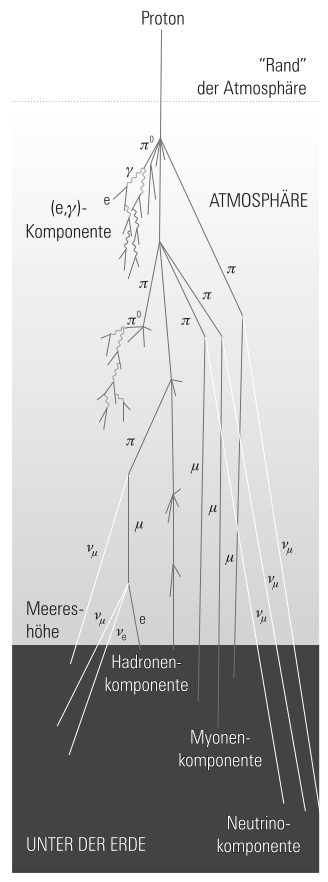
\includegraphics[width=0.5\textwidth]{bilder/zerfall.png}
    \caption{Dargestellt ist der anschauliche Zerfall eines Protons bei Eintritt in die Atmosphäre. 
            Deutlich zu sehen sind die einzelnen Zerfallspartner aus denen schließlich Myonen entstehen \cite{einfuehrung}.}
    \label{ehhnicht}
\end{figure}

\newpage
\subsection{Szintillator}
\label{szin}
Unter einem Szintillator versteht man einen bestimmten Detektortyp, welcher sich in einigen Anwendungsgebieten als Vorteilhaft herausstellt. Dies gilt ebenfalls für das
Detektieren von kosmischen Myonen. 
\\
Die allgemeine Funktionsweise beruht auf der Ionisation des verwendeten Szintillatorstoffes durch die zu untersuchende Strahlung. In Szintillatoren können je nach Bauart, Teilchen und auch elektromagnetische Strahlung 
gemessen werden. Durch die Ionisation kommt es zur Anregung des Szintillatorstoffes und anschließend zur Fluoreszenz. Wichtig hierbei ist, dass der Szintillator selbstdurchlässig für das ausgesendete Licht ist. Sonst würde
das zu messende Licht vom Stoff selbst nahezu vollständig absorbiert werden. Um dies zu verhindern wird meist an Aktivatorstoff (Wellenlängenschieber) verwendet.
\\
In der Regel wird zwischen zwei Hauptgruppen von Szintillatoren unterschieden, den anorganischen und organischen Szintillatoren.
\\
\newline
Anorganische Szintillatoren sind häufig Kristalle mit deutlich höhreren Ordnungszahlen im Vergleich zu organischen Stoffen. Die Folge dessen ist
meist eine längere Dauer bis sich die Moleküle im Kristall abgeregt haben. Für die Untersuchung der Lebensdauer von Myonen muss eine geringe Totzeit des
Szintillators gewährleistet sein, wodurch diese Art von Szintillatoren meist ungünstig sind.
\\
\newline
Organische Szintillatoren sind oft kunststoffhaltig, oder flüssig. Da die Ereignisrate des Einfalls von Myonen im Vergleich zu anderen Strahlungsquellen eher gering ist, muss meist
auch ein großes Volumen mit dem Szintillator ausgefüllt werden. Organische Szintillatoren sind dort deutlich effizienter und kostengünstiger.
\\
\newline
Für die Signalverarbeitung wird an beiden Enden des Szintillators ein Photomultiplier verwendet. 
Die Strahlung, welche durch den Szintillator entsteht, kann über die Photomultiplier verstärkt und in ein Spannungssignal umgewandelt werden. Dazu werden 
durch die Strahlung an einer Photokathode Elektronen herausgelöst und anschließend über mehrere positiv geladenen Dynoden 
beschleunigt. An jeder Dynode wird die Anzahl der Elektronen 
vervielfacht. Am Ende des Photomultipliers ist meist ein Vorverstärker eingebaut, der die kurzen Stromimpulse über ein Kondensator in ein leichter zu messendes Spannungssignal umwandelt.

\subsection{Zerfall und Lebensdauer}
Der Zerfall eines einzelnen Myons ist ein statistischer %statisch = statistisch?
Prozess und unabhängig von der Zeit die es bereits vorliegt. Es gibt also keinen Alterungsprozess von Myonen.
Die Wahrscheinlichkeit das ein Teilchen zerfällt, lässt sich also für ein beliebig kleinen Zeitraum $\text{d}t$ als
\begin{equation}
    \label{eqn:lolol}
\text{dW} = \lambda_{\mu} \text{d}t
\end{equation}
angeben. Die Konstante $\lambda_{\mu}$ beschreibt die Zerfallswahrscheinlichkeit eines Myons pro Zeiteinheit.
Wenn nun eine Anzahl N an Myonen vorliegt, lässt sich der zeitliche Verlauf dieser durch
\begin{equation}
\text{dN} = - \text{N} \text{dW}
\end{equation}
beschreiben. Mit der Beziehung \ref{eqn:lolol} folgt nun
\begin{equation*}
\text{dN} = - \text{N} \lambda_{\mu} \text{d}t.
\end{equation*}
Diese Differentialgleichung wird gelöst durch 
\begin{equation}
    \label{eqn:lololol}
\text{N}(t) = \text{N}_0 \cdot \text{exp}(- \lambda_{\mu}t),
\end{equation}
wobei $\text{N}_0$ die Anzahl der Myonen zum Zeitpunkt $t=0$ beschreibt. Um nun eine Verteilungsfunktion zu erhalten wird eine infinitesimale
Änderung der Myonenanzahl betrachtet. Es gilt
\begin{equation}
\frac{\text{dN}(t)}{\text{N}_0} = \frac{\text{N}(t + \text{d}t) - \text{N}(t)}{\text{N}_0} = - \left(\frac{\text{dN}}{\text{d}t}\right)\frac{\text{d}t}{\text{N}_0}.
\end{equation}
Wird nun die Ableitung ausgeführt, ergibt sich eine Verteilungsfunktion welche zur Berechnung des Mittelwerts genutzt werden kann. Der Mittelwert über die Zeit 
entspricht der Lebensdauer der Myonen. Die Lebensdauer folgt also aus
\begin{equation}
    \label{eqn:123123}
    \langle t \rangle := \tau = \int_0^{\infty} t \lambda_{\mu} \text{exp}(- \lambda_{\mu} t) \text{d}t = \frac{1}{\lambda_{\mu}}.
\end{equation}
Für die Bestimmung der Lebensdauer in diesem Versuch wird die Methode der kleinsten Quadrate verwendet. Dazu werden die Individuallebenszeiten der Myonen gemessen und an 
die Anzahl dieser Lebensdauern an eine Exponentialfunktion der Form \ref{eqn:lololol} angepasst. 
Analytisch sieht dies folgendermaßen aus
\begin{equation}
\sum_{i=1}^{n} \left( \text{N}(t_i) - \text{N}_0 \cdot \text{exp}(- \lambda_{\mu}t_i)\right)^2 \stackrel{!}{=} \text{min}
\end{equation}
Dies lässt sich durch eine bestimmte Wahl von $\lambda_{\mu}$ und $\text{N}_0$ minimieren, woraus auch $\tau$ über Beziehung \ref{eqn:123123} berechnet werden kann.